% Generated by make_fig_overview.py from the Bugs4Q original and the tool's output. Do not edit by hand.
\documentclass[tikz,border=2pt]{standalone}
\usepackage[T1]{fontenc}
\usepackage{newtxtext,newtxmath}
\usepackage[varqu,scaled=0.95]{zi4}
\usetikzlibrary{arrows.meta,positioning,calc,backgrounds,fit}
\definecolor{ink}{HTML}{1F2328}\definecolor{mute}{HTML}{6E7781}\definecolor{rule}{HTML}{D0D7DE}
\definecolor{wire}{HTML}{0969DA}\definecolor{wireL}{HTML}{DDEBFF}
\definecolor{fault}{HTML}{CF4A1B}\definecolor{faultL}{HTML}{FCE4DA}
\definecolor{pdg}{HTML}{8C959F}\definecolor{hlC}{HTML}{FFF1B8}\definecolor{tree}{HTML}{6639BA}\definecolor{treeL}{HTML}{F1EAFE}
\tikzset{
  >={Stealth[length=3.6pt,width=3.2pt]},
  stage/.style={font=\footnotesize\bfseries, text=ink, anchor=south west, inner sep=0pt},
  stnum/.style={circle, draw=ink, line width=0.6pt, font=\scriptsize\bfseries, text=ink, inner sep=0pt, minimum size=9pt},
  code/.style={font=\ttfamily\fontsize{5.8}{8}\selectfont, text=ink, anchor=west, inner sep=0pt},
  lno/.style={font=\ttfamily\fontsize{5.8}{8}\selectfont, text=mute, anchor=east, inner sep=0pt},
  xn/.style={rectangle, rounded corners=1.6pt, draw=tree, fill=treeL, line width=0.5pt,
        font=\ttfamily\fontsize{6}{7}\selectfont, text=ink, inner xsep=2.2pt, inner ysep=1.6pt},
  xleaf/.style={font=\ttfamily\fontsize{6}{7}\selectfont, text=ink, inner sep=1pt},
  gnode/.style={rectangle, rounded corners=1.5pt, line width=0.55pt, font=\ttfamily\fontsize{6}{6.8}\selectfont, text=ink,
        inner xsep=2pt, inner ysep=1.4pt, align=center},
  gate/.style={rectangle, draw=ink, fill=white, line width=0.55pt, minimum size=11pt, inner sep=0pt,
        font=\fontsize{7}{8}\selectfont},
  xml/.style={font=\ttfamily\fontsize{6}{6.8}\selectfont, anchor=west, inner sep=0pt},
  note/.style={font=\fontsize{6.4}{7.6}\selectfont\itshape, execute at begin node={\hyphenpenalty=10000\exhyphenpenalty=10000}, text=mute, align=center, inner sep=1pt},
  flowarrow/.style={->, line width=0.7pt, draw=ink},
}
\newcommand{\hlbox}[1]{{\setlength{\fboxsep}{0.5pt}\colorbox{hlC}{\strut #1}}}
\newcommand{\hlm}[1]{\raisebox{0.9ex}{\textcolor{tree}{\fontsize{5.4}{6}\selectfont\bfseries\rmfamily #1}}}
\newcommand{\hl}[1]{\textcolor{tree}{\bfseries #1}}
\begin{document}
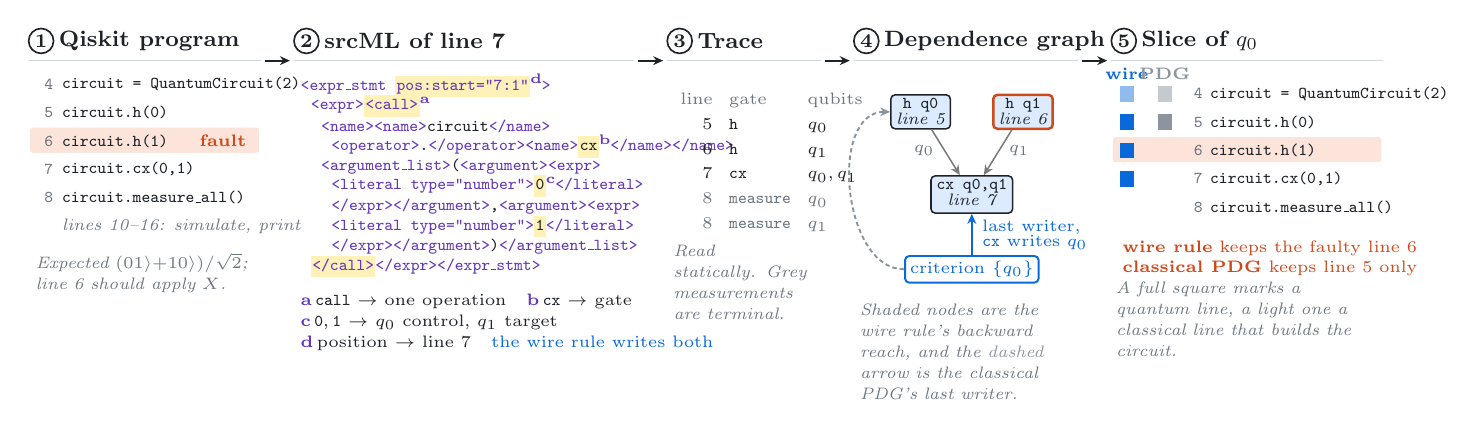
\begin{tikzpicture}

\node[stnum] (n1) at (0.16,0.55) {1};
\node[stage, anchor=west] at (0.38,0.55) {Qiskit program};
\draw[rule, line width=0.6pt] (0.0,0.3) -- (2.95,0.3);
\node[lno] at (0.32,0.0) {4};
\node[code] at (0.42,0.0) {circuit = QuantumCircuit(2)};
\node[lno] at (0.32,-0.36) {5};
\node[code] at (0.42,-0.36) {circuit.h(0)};
\fill[faultL, rounded corners=1pt] (0.02,-0.87) rectangle (2.93,-0.5499999999999999);
\node[lno] at (0.32,-0.72) {6};
\node[code] at (0.42,-0.72) {circuit.h(1)};
\node[lno] at (0.32,-1.08) {7};
\node[code] at (0.42,-1.08) {circuit.cx(0,1)};
\node[lno] at (0.32,-1.44) {8};
\node[code] at (0.42,-1.44) {circuit.measure\_all()};
\node[font=\fontsize{6.2}{7}\selectfont\bfseries, text=fault, anchor=east] at (2.89,-0.72) {fault};
\node[code, text=mute] at (0.42,-1.7999999999999998) {\itshape\rmfamily\fontsize{6.3}{8}\selectfont lines 10--16: simulate, print};
\node[note, anchor=north west, align=left, text width=2.85cm] at (0.05,-2.0999999999999996) {Expected $(\lvert01\rangle{+}\lvert10\rangle)/\sqrt{2}$; line~6 should apply $X$.};
\node[stnum] (n2) at (3.5300000000000002,0.55) {2};
\node[stage, anchor=west] at (3.75,0.55) {srcML of line 7};
\draw[rule, line width=0.6pt] (3.37,0.3) -- (7.69,0.3);
\node[xml] at (3.45,-0.02) {\textcolor{tree}{<expr\_stmt \hlbox{pos:start="7:1"}\hlm{d}>}};
\node[xml] at (3.58,-0.275) {\textcolor{tree}{<expr>}\textcolor{tree}{\hlbox{<call>}\hlm{a}}};
\node[xml] at (3.71,-0.53) {\textcolor{tree}{<name>}\textcolor{tree}{<name>}\textcolor{ink}{\bfseries circuit}\textcolor{tree}{</name>}};
\node[xml] at (3.8400000000000003,-0.785) {\textcolor{tree}{<operator>}\textcolor{ink}{\bfseries .}\textcolor{tree}{</operator>}\textcolor{tree}{<name>}\hlbox{\textcolor{ink}{\bfseries cx}}\hlm{b}\textcolor{tree}{</name>}\textcolor{tree}{</name>}};
\node[xml] at (3.71,-1.04) {\textcolor{tree}{<argument\_list>}\textcolor{ink}{\bfseries (}\textcolor{tree}{<argument>}\textcolor{tree}{<expr>}};
\node[xml] at (3.8400000000000003,-1.295) {\textcolor{tree}{<literal type="number">}\hlbox{\textcolor{ink}{\bfseries 0}}\hlm{c}\textcolor{tree}{</literal>}};
\node[xml] at (3.8400000000000003,-1.55) {\textcolor{tree}{</expr>}\textcolor{tree}{</argument>}\textcolor{ink}{\bfseries ,}\textcolor{tree}{<argument>}\textcolor{tree}{<expr>}};
\node[xml] at (3.8400000000000003,-1.8050000000000002) {\textcolor{tree}{<literal type="number">}\hlbox{\textcolor{ink}{\bfseries 1}}\textcolor{tree}{</literal>}};
\node[xml] at (3.8400000000000003,-2.06) {\textcolor{tree}{</expr>}\textcolor{tree}{</argument>}\textcolor{ink}{\bfseries )}\textcolor{tree}{</argument\_list>}};
\node[xml] at (3.58,-2.315) {\textcolor{tree}{\hlbox{</call>}}\textcolor{tree}{</expr>}\textcolor{tree}{</expr\_stmt>}};
\node[anchor=north west, align=left, font=\fontsize{6.2}{7.6}\selectfont, text=ink, inner sep=0pt] at (3.45,-2.65) {\hl{a}\,\texttt{call} $\to$ one operation\quad \hl{b}\,\texttt{cx} $\to$ gate\\\hl{c}\,\texttt{0},\,\texttt{1} $\to$ $q_{0}$ control, $q_{1}$ target\\\hl{d}\,position $\to$ line 7\quad \textcolor{wire}{the wire rule writes both}};
\node[stnum] (n3) at (8.270000000000001,0.55) {3};
\node[stage, anchor=west] at (8.490000000000002,0.55) {Trace};
\draw[rule, line width=0.6pt] (8.110000000000001,0.3) -- (10.06,0.3);
\node[anchor=north west, font=\fontsize{6.4}{8}\selectfont, text=ink, inner sep=0pt] at (8.170000000000002,-0.05) {\setlength{\tabcolsep}{3pt}\begin{tabular}{rll}\textcolor{mute}{line}&\textcolor{mute}{gate}&\textcolor{mute}{qubits}\\[1pt]5&\texttt{h}&$q_0$\\[1pt]6&\texttt{h}&$q_1$\\[1pt]7&\texttt{cx}&$q_0$,\,$q_1$\\[1pt]\textcolor{mute}{8}&\textcolor{mute}{\texttt{measure}}&\textcolor{mute}{$q_0$}\\[1pt]\textcolor{mute}{8}&\textcolor{mute}{\texttt{measure}}&\textcolor{mute}{$q_1$}\\[1pt]\end{tabular}};
\node[note, anchor=north west, align=left, text width=1.8499999999999999cm] at (8.15,-2.0) {Read statically. Grey measurements are terminal.};
\node[stnum] (n4) at (10.64,0.55) {4};
\node[stage, anchor=west] at (10.860000000000001,0.55) {Dependence graph};
\draw[rule, line width=0.6pt] (10.48,0.3) -- (13.33,0.3);
\node[gnode, fill=wireL, draw=ink] (g0) at (11.330000000000002,-0.35) {h q0\\[-1pt]{\rmfamily\itshape\fontsize{5.6}{6}\selectfont line 5}};
\node[gnode, fill=wireL, draw=fault, line width=0.9pt] (g1) at (12.63,-0.35) {h q1\\[-1pt]{\rmfamily\itshape\fontsize{5.6}{6}\selectfont line 6}};
\node[gnode, fill=wireL, draw=ink] (g2) at (11.98,-1.4) {cx q0,q1\\[-1pt]{\rmfamily\itshape\fontsize{5.6}{6}\selectfont line 7}};
\draw[->, draw=ink!60, line width=0.55pt] (g0) -- node[left, pos=0.45, font=\fontsize{5.6}{6}\selectfont, text=mute] {$q_0$} (g2);
\draw[->, draw=ink!60, line width=0.55pt] (g1) -- node[right, pos=0.45, font=\fontsize{5.6}{6}\selectfont, text=mute] {$q_1$} (g2);
\node[rectangle, rounded corners=1.5pt, draw=wire, line width=0.7pt, font=\fontsize{6.3}{7}\selectfont, text=wire, inner sep=1.8pt] (crit) at (11.98,-2.35) {criterion $\{q_0\}$};
\draw[->, wire, line width=0.9pt] (crit) -- node[right, font=\fontsize{5.6}{6.4}\selectfont, text=wire, align=left] {last writer,\\[-1pt]\texttt{cx} writes $q_0$} (g2);
\draw[->, pdg, line width=0.7pt, dash pattern=on 1.6pt off 1.1pt] (crit.west) to[out=180, in=180] (g0.west);
\node[note, anchor=north west, align=left, text width=2.75cm] at (10.52,-2.75) {Shaded nodes are the wire rule's backward reach, and the \textcolor{pdg}{dashed} arrow is the classical PDG's last writer.};
\node[stnum] (n5) at (13.91,0.55) {5};
\node[stage, anchor=west] at (14.13,0.55) {Slice of $q_0$};
\draw[rule, line width=0.6pt] (13.75,0.3) -- (17.2,0.3);
\node[font=\fontsize{5.8}{6.5}\selectfont\bfseries, text=wire] at (13.95,0.13) {wire};
\node[font=\fontsize{5.8}{6.5}\selectfont\bfseries, text=pdg] at (14.43,0.13) {PDG};
\fill[wire!45] (13.86,-0.22) rectangle (14.04,-0.01999999999999999);
\fill[pdg!50] (14.34,-0.22) rectangle (14.52,-0.01999999999999999);
\node[lno] at (14.92,-0.12) {4};
\node[code] at (15.0,-0.12) {circuit = QuantumCircuit(2)};
\fill[wire] (13.86,-0.58) rectangle (14.04,-0.38);
\fill[pdg] (14.34,-0.58) rectangle (14.52,-0.38);
\node[lno] at (14.92,-0.48) {5};
\node[code] at (15.0,-0.48) {circuit.h(0)};
\fill[faultL, rounded corners=1pt] (13.77,-0.99) rectangle (17.18,-0.6699999999999999);
\fill[wire] (13.86,-0.94) rectangle (14.04,-0.74);
\node[lno] at (14.92,-0.84) {6};
\node[code] at (15.0,-0.84) {circuit.h(1)};
\fill[wire] (13.86,-1.3000000000000003) rectangle (14.04,-1.1);
\node[lno] at (14.92,-1.2000000000000002) {7};
\node[code] at (15.0,-1.2000000000000002) {circuit.cx(0,1)};
\node[lno] at (14.92,-1.56) {8};
\node[code] at (15.0,-1.56) {circuit.measure\_all()};
\node[font=\fontsize{6.2}{7}\selectfont, text=fault, anchor=north west, align=left] at (13.77,-1.8699999999999999) {\textbf{wire rule} keeps the faulty line~6\\\textbf{classical PDG} keeps line~5 only};
\node[note, anchor=north west, align=left, text width=3.35cm] at (13.77,-2.4699999999999998) {A full square marks a quantum line, a light one a classical line that builds the circuit.};
\draw[flowarrow] (3.0,0.3) -- (3.3200000000000003,0.3);
\draw[flowarrow] (7.74,0.3) -- (8.06,0.3);
\draw[flowarrow] (10.110000000000001,0.3) -- (10.43,0.3);
\draw[flowarrow] (13.38,0.3) -- (13.7,0.3);
\end{tikzpicture}
\end{document}
